\documentclass{article}
\usepackage{tikz}

\begin{document}
  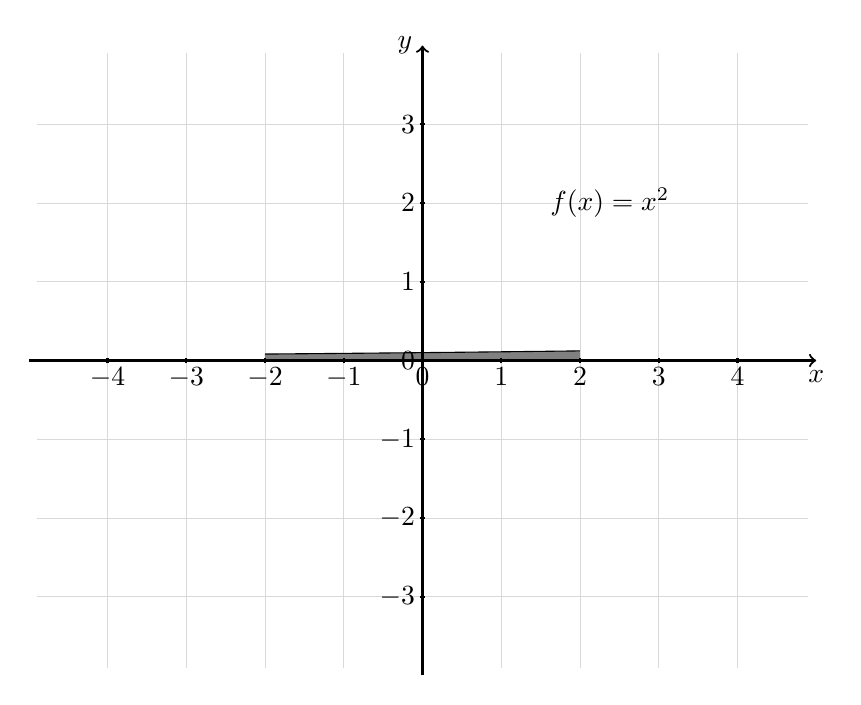
\begin{tikzpicture}
    \draw[very thin, gray!30, step=1 cm](-4.9,-3.9) grid (4.9,3.9);

    \fill [gray, domain=-2:2, variable=\x]
      (-2, 0)
      -- plot ({\x}, {(1/10) * exp(\x/10)})
      -- (2, 0)
      -- cycle;

    \draw [thick] [->] (-5,0)--(5,0) node[right, below] {$x$};
     \foreach \x in {-4,...,4}
       \draw[xshift=\x cm, thick] (0pt,-1pt)--(0pt,1pt) node[below] {$\x$};

    \draw [thick] [->] (0,-4)--(0,4) node[above, left] {$y$};
     \foreach \y in {-3,...,3}
       \draw[yshift=\y cm, thick] (-1pt,0pt)--(1pt,0pt) node[left] {$\y$};

    \draw [domain=-2:2, variable=\x]
      plot ({\x}, {(1/10) * exp(\x/10)}) node[right] at (1.5,2) {$f(x)=x^2$};

  \end{tikzpicture}
\end{document}
